\documentclass[aspectratio=169]{beamer}

\usetheme{default}
\setbeamertemplate{navigation symbols}{}
\setbeamertemplate{itemize item}{\color{black}\textbullet}
\setbeamertemplate{itemize subitem}{\color{black}\textbullet}
\usepackage{xcolor}
\definecolor{navy}{RGB}{0, 0, 128}

\begin{document}

\begin{frame}

Start with the research question and data structure

\bigskip

\onslide<2->{
Random Coefficients: Use when heterogeneity is continuous
\bigskip

\begin{itemize}
\item Willingness-to-pay distributions
\item[] 
\item Individual-specific elasticities
\end{itemize}
}

\bigskip

\onslide<3->{
Finite Mixtures: Use when heterogeneity is discrete
\bigskip

\begin{itemize}
\item Market segmentation
\item[]
\item Behavioral types (e.g., price-sensitive vs quality-focused)
\end{itemize}
}

\bigskip

\onslide<4->{
Does the economic theory suggest continuous or discrete heterogeneity?
}

\end{frame}



\begin{frame}

Likelihood surfaces are highly non-concave with heterogeneity

\bigskip

\onslide<2->{
Solutions:
\bigskip
\begin{itemize}
\item Multiple random starting values (minimum 50-100)
\item[] 
\item Grid search over key parameters
\item[]
\item Use simpler model estimates as starting values
\end{itemize}
}

\bigskip

\onslide<3->{
Diagnostic: Compare final likelihood across different starts
}

\bigskip

\onslide<4->{
If estimates vary dramatically, increase number of starting values or simplify specification
}

\end{frame}

\begin{frame}

More parameters $\neq$ better model

\bigskip

\onslide<2->{
Warning Signs:
\bigskip

\begin{itemize}
\item Very small estimated mixing probabilities ($< 0.05$)
\item[] 
\item Nearly identical parameter vectors across types
\item[]
\item Unstable estimates across samples
\end{itemize}
}

\bigskip

\onslide<4->{
Start simple and build complexity gradually
}

\end{frame}

\begin{frame}

For finite mixture models: How many types $K$?

\bigskip

\onslide<2->{
Statistical Approach:
\begin{align*}
\text{Choose } K \text{ to minimize: } \text{BIC} = -2\mathcal{L} + k\ln(n)
\end{align*}
}

\onslide<3->{
Economic Approach:
\bigskip

\begin{itemize}
\item Do additional types reveal meaningful segments?
\item[]
\item Can you interpret and name each type?
\end{itemize}
}

\bigskip

\onslide<4->{
Practical constraint: Rarely use more than 4-5 types in practice
}

\end{frame}

\begin{frame}

How do you know the algorithm has converged?

\bigskip

\onslide<2->{
Standard criterion:
\begin{align*}
\frac{|\mathcal{L}^{(t+1)} - \mathcal{L}^{(t)}|}{|\mathcal{L}^{(t)}|} < \text{tolerance}
\end{align*}
}

\onslide<3->{
Additional checks:
\bigskip

\begin{itemize}
\item Parameter stability across iterations
\item[] 
\item Multiple starting values reach same solution
\item[] 
\item Gradient near zero (for Newton-type methods)
\end{itemize}
}

\bigskip

\onslide<4->{
Be suspicious of ``convergence'' after very few iterations
}

\end{frame}


\begin{frame}
    \centering
    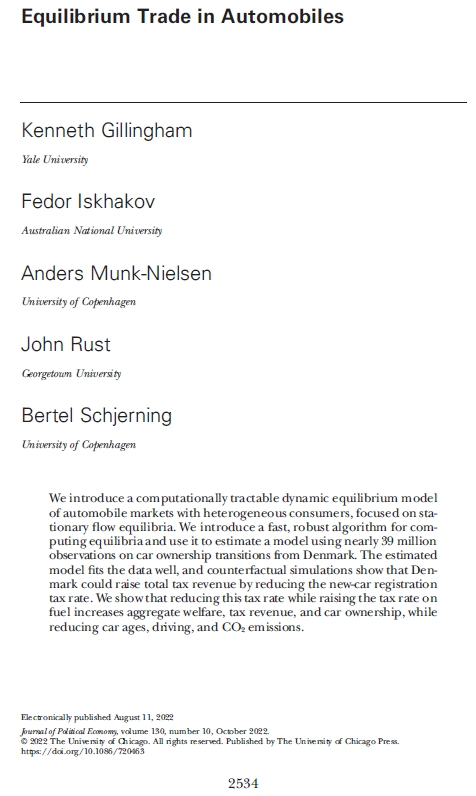
\includegraphics[width=0.35\textwidth]{gillingham_cover.jpg}
\end{frame}



\begin{frame}

\onslide<1->{
Problem: Analyze car tax policy with 39 million observations
}

\bigskip

\onslide<2->{
Approach: 
\bigskip

\begin{itemize}
    \item 8 (observable) household types, 4 car types, 25 age categories
    \item[]
    \item Nested Logit GEV
    \item[] 
    \item Complicated dynamic market equilibrium
\end{itemize}
}

\bigskip

\onslide<3->{
Key finding: ``Hand-me-down chain'' from rich to poor households
}

\bigskip

\onslide<4->{
Policy insight: Current registration tax above Laffer curve peak
}

\end{frame}


\end{document}